\documentclass{beamer}

\usepackage[utf8]{inputenc}
\usepackage[T1]{fontenc}
\usepackage[ngerman]{babel}
\usepackage{graphicx} % Bilder
\usepackage{wrapfig} % Umflussbilder
\usepackage{multicol} % Multiple columns
\usepackage{minted} % Haskell source code
\usepackage{framed} % Frames around source code
\usepackage[framemethod=tikz]{mdframed} % Frames
\usepackage{verbatim} % \begin{comment}...\end{comment}
\usepackage{etoolbox} % manipulate minted
\AtBeginEnvironment{minted}{\fontsize{10}{10}\selectfont}
\AfterEndEnvironment{minted}{}

\mdfdefinestyle{fancy}{
  roundcorner=5pt,
  linewidth=4pt,
  linecolor=red!80,
  backgroundcolor=red!20
}
\newmdenv[style=fancy]{important}

% redifine \em for \emph to use bold instead of italics
\makeatletter
\DeclareRobustCommand{\em}{%
  \@nomath\em \if b\expandafter\@car\f@series\@nil
  \normalfont \else \bfseries \fi}
\makeatother

% Stuff for Beamer
\beamertemplatenavigationsymbolsempty
\usetheme{Warsaw}

\title{Fortgeschrittene Funktionale Programmierung in Haskell}

\begin{document}
  
%----------------------------------------------------------------------------------------  

  \begin{frame}
  \begin{center}
    \huge\textbf{Fortgeschrittene Funktionale Programmierung in Haskell}\\ \bigskip
    \LARGE Universität Bielefeld, Sommersemester 2015\\ \bigskip
    \large Jonas Betzendahl \& Stefan Dresselhaus
    \end{center}
  \end{frame}

%----------------------------------------------------------------------------------------  

\begin{frame}[allowframebreaks]{Outline}
\frametitle{Übersicht}
\tableofcontents
\end{frame}

%----------------------------------------------------------------------------------------
\section*{Alligator Eggs}
%----------------------------------------------------------------------------------------

\begin{frame}

\begin{center}
\Large \textbf{Alligator Eggs} \tiny \bigskip

Idee \& Bilder: Bret Victor\\
\texttt{http://worrydream.com/AlligatorEggs/}
\end{center}

\end{frame}

%----------------------------------------------------------------------------------------
\subsection*{Konzept}

\begin{frame}
Wir betrachten heute ein Spiel, das gleichzeitig bunt und putzig ist und uns erlaubt,
etwas interessantes zu lernen! Es gibt\dots \pause\smallskip

\begin{itemize}
\item \textbf{Hungrige Alligatoren}\\
      
\includegraphics[scale=0.2]{pieces_1.png}\\
      Hungrige Alligatoren sind hungrig! Sie fressen alles, was ihnen vor's Maul kommt.
      Sie bewachen aber außerdem ihre Familien.
      \pause
\item \textbf{Alte Alligatoren}\\
      
\includegraphics[scale=0.2]{pieces_2.png}\\
      Diese Alligatoren haben genug gegessen und bewachen nur noch ihre Familien.
      \pause
\item \textbf{Alligatoreier}\\
      
\includegraphics[scale=0.2]{pieces_3.png}\\
      Aus Eiern schlüpfen demnächst neue Alligatorfamilien.
\end{itemize}

\end{frame}

%----------------------------------------------------------------------------------------

\begin{frame}
\frametitle{Familien}

Alligatoren kommen in Familien daher. Hier ist eine:

\begin{multicols}{2}

\begin{center}
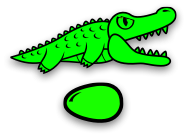
\includegraphics[scale=0.6]{families_1.png} 
\end{center}

\columnbreak
\pause

Hier ist noch nicht viel zu sehen, was wirklich interessiert.\smallskip\smallskip

Nur ein grüner Alligator, der sein grünes Ei bewacht.\\Ist er nicht süß?

\end{multicols}

\end{frame}

%----------------------------------------------------------------------------------------

\begin{frame}
\frametitle{Familien}

Hier ist eine weitere Familie, dieses Mal mit mehr Mitgliedern.\pause

\begin{multicols}{2}

\begin{center}
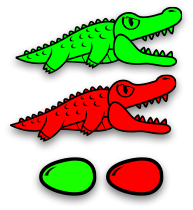
\includegraphics[scale=0.6]{families_2.png} 
\end{center}

\columnbreak

Ein grüner und ein roter Alligator bewachen ein grünes und ein rotes Ei.\bigskip

Oder anders formuliert:

Ein grüner Alligator bewacht einen roten Alligator und der rote Alligator bewacht die zwei Eier.

\end{multicols}

\end{frame}

%----------------------------------------------------------------------------------------

\begin{frame}
\frametitle{Familien}

Dieses Mal haben wir eine richtige Großfamilie:\pause

\begin{multicols}{2}

\begin{center}
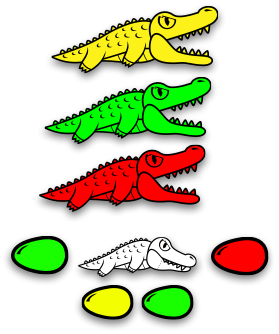
\includegraphics[scale=0.5]{families_3.png} 
\end{center}

\columnbreak
\pause

Hier haben wir drei hungrige Alligatoren, die Wache halten. Einen gelben, einen grünen und einen roten.\pause\bigskip

Sie bewachen drei Dinge: Ein grünes Ei, einen alten Alligator und ein rotes Ei.\pause\bigskip

Der alte Alligator hingegen bewacht ein gelbes und ein grünes Ei. 

\end{multicols}

\end{frame}

%----------------------------------------------------------------------------------------
\subsection*{Beispiel}

\begin{frame}
\frametitle{Fressen und gefressen werden}

\begin{center}
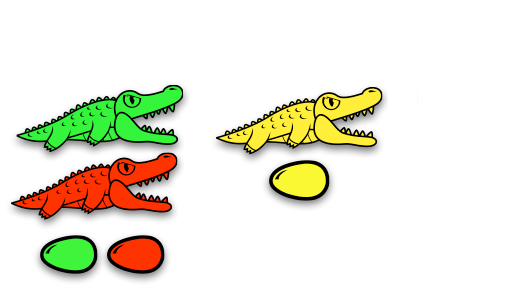
\includegraphics[scale=0.45]{eating_1.png} 
\end{center}
\bigskip

Hier wird es etwas ungemütlicher. Wir sehen hier zwei Familien nebeneinander.
\end{frame}

%----------------------------------------------------------------------------------------

\begin{frame}
\frametitle{Fressen und gefressen werden}

\begin{center}
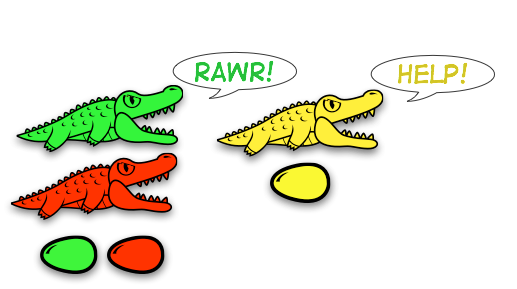
\includegraphics[scale=0.45]{eating_2.png} 
\end{center}
\bigskip

Hier wird es etwas ungemütlicher. Wir sehen hier zwei Familien nebeneinander. Der grüne Alligator ist \emph{sehr} hungrig\dots
\end{frame}

%----------------------------------------------------------------------------------------

\begin{frame}
\frametitle{Fressen und gefressen werden}

\begin{center}
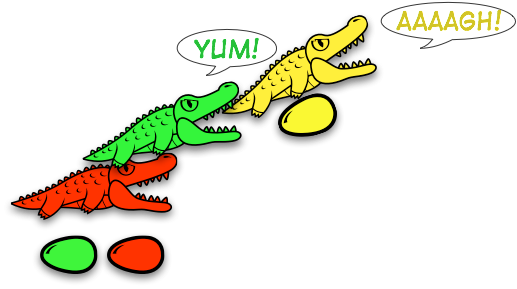
\includegraphics[scale=0.45]{eating_3.png} 
\end{center}
\bigskip

Hier wird es etwas ungemütlicher. Wir sehen hier zwei Familien nebeneinander. Der grüne Alligator ist \emph{sehr} hungrig\dots
\end{frame}

%----------------------------------------------------------------------------------------

\begin{frame}
\begin{multicols}{2}
\frametitle{Fressen und gefressen werden}

\begin{center}
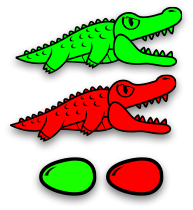
\includegraphics[scale=0.45]{families_2.png} 
\end{center}
\columnbreak

Der grüne Alligator hat die komplette gelbe Familie gefressen.

\end{multicols}
\end{frame}

%----------------------------------------------------------------------------------------

\begin{frame}
\begin{multicols}{2}
\frametitle{Fressen und gefressen werden}

\begin{center}
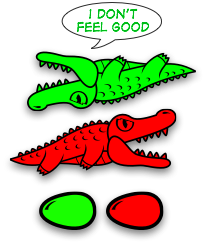
\includegraphics[scale=0.45]{eating_4.png} 
\end{center}
\columnbreak

Der grüne Alligator hat die komplette gelbe Familie gefressen. Das war allerdings zu viel für seinen Magen. Er hat sich überfressen und stirbt.

\end{multicols}
\end{frame}

%----------------------------------------------------------------------------------------

\begin{frame}
\begin{multicols}{2}
\frametitle{Fressen und gefressen werden}

\begin{center}
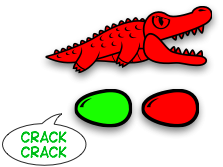
\includegraphics[scale=0.45]{eating_5.png} 
\end{center}
\columnbreak

Was übrig bleibt ist der rote Alligator. Jetzt wo sein grüner Freund gestorben ist, fängt jedoch das grüne Ei an, zu schlüpfen.

\end{multicols}
\end{frame}

%----------------------------------------------------------------------------------------

\begin{frame}
\begin{multicols}{2}
\frametitle{Fressen und gefressen werden}

\begin{center}
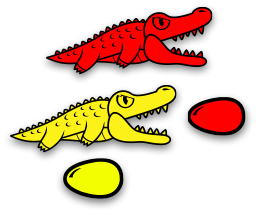
\includegraphics[scale=0.45]{eating_6.png} 
\end{center}
\columnbreak

Was übrig bleibt ist der rote Alligator. Jetzt wo sein grüner Freund gestorben ist, fängt jedoch das grüne Ei an, zu schlüpfen.

Es schlüpft \emph{exakt}, was der grüne Alligator gerade gegessen hat. Das Wunder des Lebens!

\end{multicols}
\end{frame}

%----------------------------------------------------------------------------------------

\begin{frame}
\begin{multicols}{2}
\frametitle{Fressen und gefressen werden}

\begin{center}
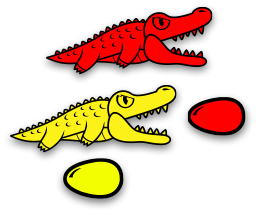
\includegraphics[scale=0.45]{eating_6.png} 
\end{center}
\columnbreak

Was übrig bleibt ist der rote Alligator. Jetzt wo sein grüner Freund gestorben ist, fängt jedoch das grüne Ei an, zu schlüpfen.

Es schlüpft \emph{exakt}, was der grüne Alligator gerade gegessen hat. Das Wunder des Lebens!

\end{multicols}
\end{frame}

%----------------------------------------------------------------------------------------

\begin{frame}
\begin{multicols}{2}
\frametitle{Fressen und gefressen werden}

\begin{center}
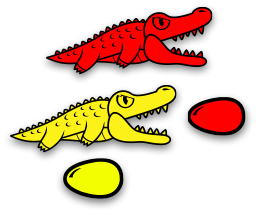
\includegraphics[scale=0.45]{eating_6.png} 
\end{center}
\columnbreak

Jetzt ist also eine neue gelbe Familie geschlüpft. 

\end{multicols}
\end{frame}


%----------------------------------------------------------------------------------------

\begin{frame}
\begin{multicols}{2}
\frametitle{Fressen und gefressen werden}

\begin{center}
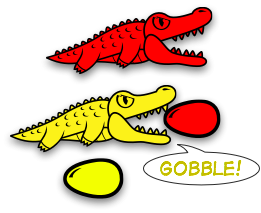
\includegraphics[scale=0.45]{eating_7.png} 
\end{center}
\columnbreak

Jetzt ist also eine neue gelbe Familie geschlüpft. Allerdings ist dieser gelbe Alligator auch ziemlich hungrig\dots

\end{multicols}
\end{frame}

%----------------------------------------------------------------------------------------

\begin{frame}
\begin{multicols}{2}
\frametitle{Fressen und gefressen werden}

\begin{center}
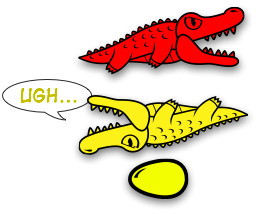
\includegraphics[scale=0.45]{eating_8.png} 
\end{center}
\columnbreak

Jetzt ist also eine neue gelbe Familie geschlüpft. Allerdings ist dieser gelbe Alligator auch ziemlich hungrig\dots

Nachdem er das rote Ei gefressen hat, ist allerdings auch sein Magen schon zu voll und ihn ereilt das gleiche Schicksal wie den grünen Alligator.

\end{multicols}
\end{frame}

%----------------------------------------------------------------------------------------

\begin{frame}
\begin{multicols}{2}
\frametitle{Fressen und gefressen werden}

\begin{center}
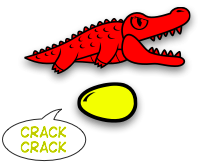
\includegraphics[scale=0.45]{eating_9.png} 
\end{center}
\columnbreak

Jetzt ist also eine neue gelbe Familie geschlüpft. Allerdings ist dieser gelbe Alligator auch ziemlich hungrig\dots

Nachdem er das rote Ei gefressen hat, ist allerdings auch sein Magen schon zu voll und ihn ereilt das gleiche Schicksal wie den grünen Alligator. Und auch aus diesem Ei schlüpft, was gerade gegessen wurde.

\end{multicols}
\end{frame}

%----------------------------------------------------------------------------------------

\begin{frame}
\begin{multicols}{2}
\frametitle{Fressen und gefressen werden}

\begin{center}
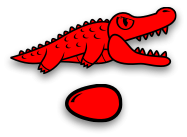
\includegraphics[scale=0.45]{eating_10.png} 
\end{center}
\columnbreak

Jetzt ist also eine neue gelbe Familie geschlüpft. Allerdings ist dieser gelbe Alligator auch ziemlich hungrig\dots

Nachdem er das rote Ei gefressen hat, ist allerdings auch sein Magen schon zu voll und ihn ereilt das gleiche Schicksal wie den grünen Alligator. Und auch aus diesem Ei schlüpft, was gerade gegessen wurde.

Hier endet das Drama, da es nichts mehr zum Fressen gibt.

\end{multicols}
\end{frame}

%----------------------------------------------------------------------------------------
\subsection*{Formale Regeln}

\begin{frame}
\frametitle{Die Essensregel}

Wir können jetzt eine erste \glqq formale\grqq\ Regel für dieses System aufstellen:\bigskip\pause

Wenn wir Alligatorfamilien nebeneinander haben, \dots\bigskip

\begin{center}
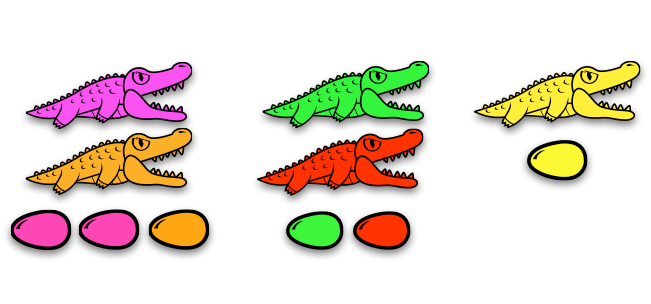
\includegraphics[scale=0.35]{eatingrule_1.png} 
\end{center}

\end{frame}

%----------------------------------------------------------------------------------------

\begin{frame}
\frametitle{Die Essensregel}

Wir können jetzt eine erste \glqq formale\grqq\ Regel für dieses System aufstellen:\bigskip

Wenn wir Alligatorfamilien nebeneinander haben, frisst der Alligator links oben die Familie rechts neben ihm.\bigskip

\begin{center}
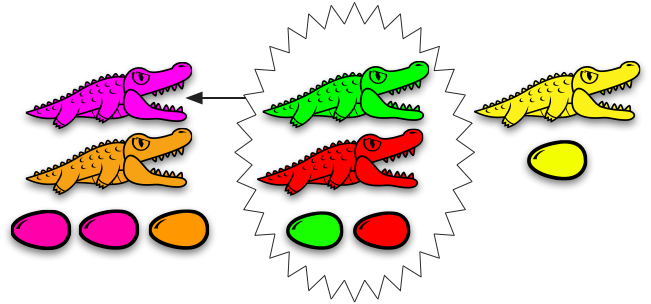
\includegraphics[scale=0.35]{eatingrule_2.png} 
\end{center}

\end{frame}

%----------------------------------------------------------------------------------------

\begin{frame}
\frametitle{Die Essensregel}

Wenn wir Alligatorfamilien nebeneinander haben, frisst der Alligator links oben die Familie rechts neben ihm. Dieser Alligator stirbt. Bewacht seine Familie jedoch Eier seiner Farbe, schlüpft aus \emph{jedem} dieser Eier, was er gerade noch verspeist hat.

\begin{center}
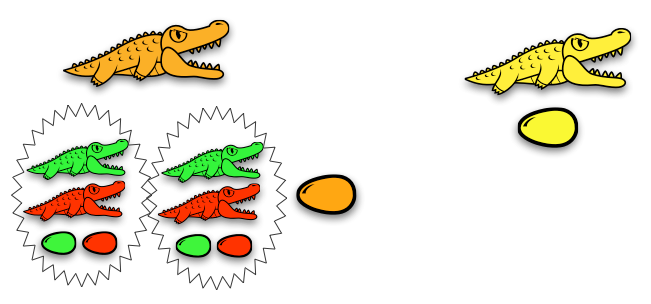
\includegraphics[scale=0.4]{eatingrule_3.png} 
\end{center}

\end{frame}

%----------------------------------------------------------------------------------------

\begin{frame}
\frametitle{Die Farbenregel}

\begin{center}
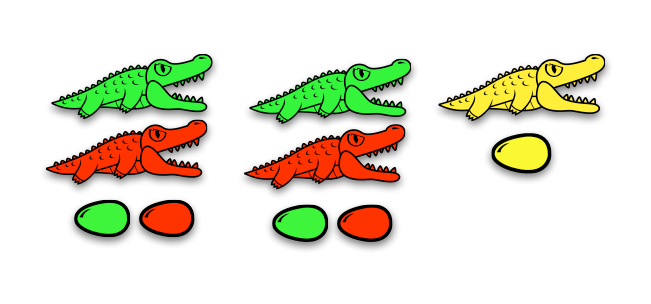
\includegraphics[scale=0.35]{eatingrule_4.png} 
\end{center}

Setzen wir das Beispiel fort, frisst Orange Gelb und wir verbleiben mit dieser Konstellation.
Jetzt gibt es allerdings ein Problem.

\end{frame}

%----------------------------------------------------------------------------------------

\begin{frame}
\frametitle{Die Farbenregel}

\begin{center}
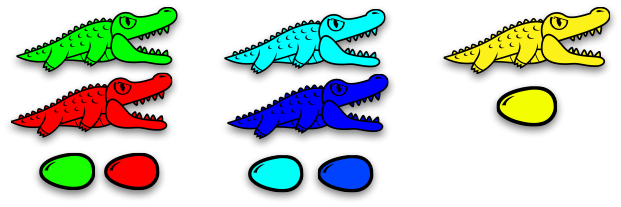
\includegraphics[scale=0.35]{colorrule_1.png} 
\end{center}

Setzen wir das Beispiel fort, frisst Orange Gelb und wir verbleiben mit dieser Konstellation.
Jetzt gibt es allerdings ein Problem.

Bevor ein Alligator eine Familie essen kann, in der eine Farbe vorkommt, die auch eins seiner Familienmitglieder hat, müssen die Farben geändert werden.

\end{frame}

%----------------------------------------------------------------------------------------

\begin{frame}
\frametitle{Die Farbenregel}

\begin{center}
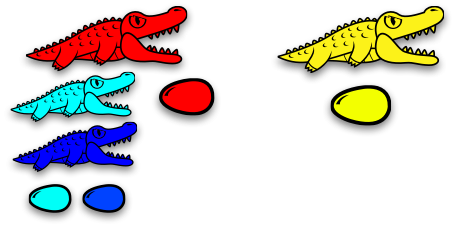
\includegraphics[scale=0.35]{colorrule_2.png} 
\end{center}

Setzen wir das Beispiel fort, frisst Orange Gelb und wir verbleiben mit dieser Konstellation.
Jetzt gibt es allerdings ein Problem.

Bevor ein Alligator eine Familie essen kann, in der eine Farbe vorkommt, die auch eins seiner Familienmitglieder hat, müssen die Farben geändert werden.

Dann können wir essen\dots

\end{frame}

%----------------------------------------------------------------------------------------

\begin{frame}
\frametitle{Die Farbenregel}

\begin{center}
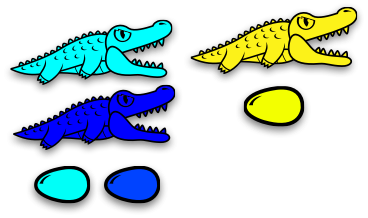
\includegraphics[scale=0.35]{colorrule_3.png} 
\end{center}

Setzen wir das Beispiel fort, frisst Orange Gelb und wir verbleiben mit dieser Konstellation.
Jetzt gibt es allerdings ein Problem.

Bevor ein Alligator eine Familie essen kann, in der eine Farbe vorkommt, die auch eins seiner Familienmitglieder hat, müssen die Farben geändert werden.

Dann können wir essen und essen\dots

\end{frame}

%----------------------------------------------------------------------------------------

\begin{frame}
\frametitle{Die Farbenregel}

\begin{center}
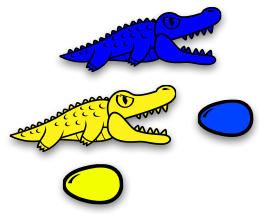
\includegraphics[scale=0.35]{colorrule_4.png} 
\end{center}

Setzen wir das Beispiel fort, frisst Orange Gelb und wir verbleiben mit dieser Konstellation.
Jetzt gibt es allerdings ein Problem.

Bevor ein Alligator eine Familie essen kann, in der eine Farbe vorkommt, die auch eins seiner Familienmitglieder hat, müssen die Farben geändert werden.

Dann können wir essen und essen und essen\dots

\end{frame}

%----------------------------------------------------------------------------------------

\begin{frame}
\frametitle{Die Farbenregel}

\begin{center}
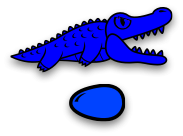
\includegraphics[scale=0.45]{colorrule_5.png} 
\end{center}

Setzen wir das Beispiel fort, frisst Orange Gelb und wir verbleiben mit dieser Konstellation.
Jetzt gibt es allerdings ein Problem.

Bevor ein Alligator eine Familie essen kann, in der eine Farbe vorkommt, die auch eins seiner Familienmitglieder hat, müssen die Farben geändert werden.

Dann können wir essen und essen und essen, bis alles weg ist.

\end{frame}

%----------------------------------------------------------------------------------------
\section*{Der Lambda-Würfel}
%----------------------------------------------------------------------------------------

%----------------------------------------------------------------------------------------
\section*{Recursion Schemes}
%----------------------------------------------------------------------------------------

%----------------------------------------------------------------------------------------

\end{document}